\appendix{}
\appendixheaderon

\section{Schematic}
\label{app:schematic}
This section shows the schematic described in Section: \ref{sec:measCirc}.

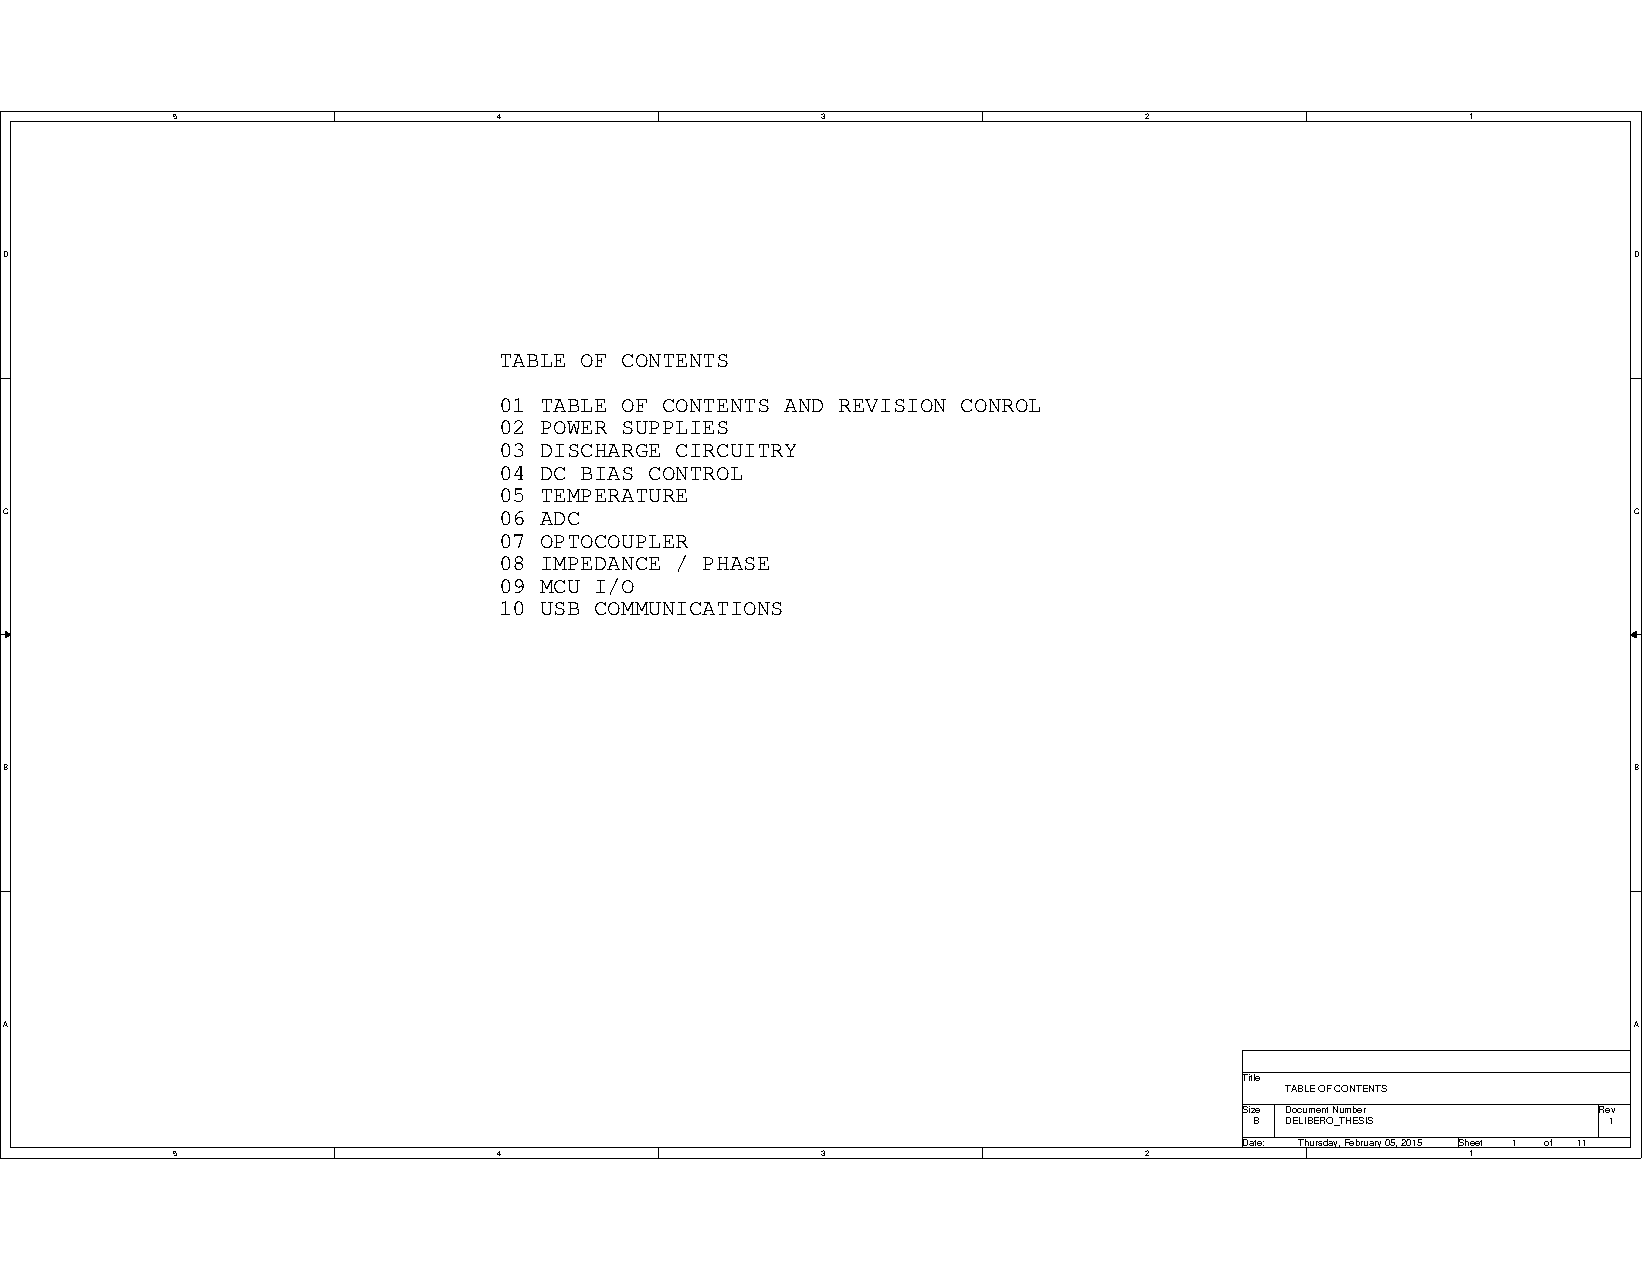
\includepdf[pages=-,angle=90,rotateoversize,offset=1.75in -.975in]{figures/board/capMeasCircuit.pdf}

\section{Generating Modeling Images}
\label{app:genModelingImages}
This appendix will list all of the matlab code and supporting files needed to generate the images seen in Section: \ref{sec:regression}.

\subsection{Example Data: Figure: \ref{fig:exCapData}}
\begin{figure}[ht!]
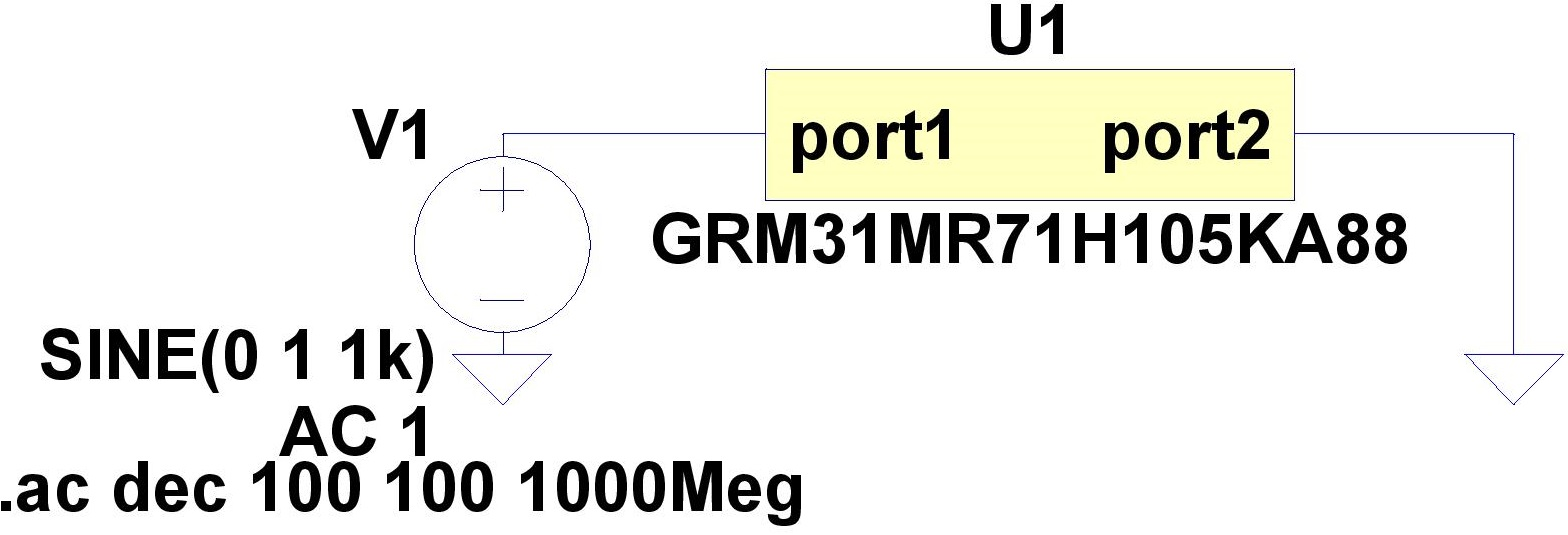
\includegraphics[keepaspectratio=true,width=2in]{./figures/appendix/exCapData_ltspice.jpg}
\centering
\caption{LTSpice Schematic for Capacitor Model}
\label{fig:exCapData_ltspice}
\end{figure}


This section will describe how to obtain and generate the example data used for the regression fitting. This method uses LTSpice to generate impedance vs frequency data from one of Murata's capacitor models. First, go to Murata's online SimSurfing tool \cite{simSurfing} and select the ``Monolic Ceramic Capacitors'' button. Download a SPICE *.mod file (Appendix: \ref{app:subcir}) for the capacitor of interest, by selecting it from the list and clicking the ``netlist'' button. Open the *.mod file in LTSpice, right click on the part name in the line starting with ``.SUBCKT,'' and select ``Create Symbol.'' Create an LTSpice schematic similar to Figure: \ref{fig:exCapData_ltspice} and plot $\frac{V(n001)}{-I(V1)}$. The negative sign is important because LTSpice defines current as coming out of a node. If the negative sign is omitted, the phase will be offset by $180^o$, and the regression analysis will solve for negative capacitance! With the plot window selected, select  $``File\rightarrow Export\rightarrow Cartesian\rightarrow OK$'' with the impedance plot selected as the waveform. Open the resultant *.txt file, delete the first line, and change all tabs to commas (``$<:>\%s/<ctrl+v><TAB>/,/g$'' , ``$\%s/\string^I/,/g$'' in vim). Make sure to save the resultant file in ``/scripts/data.''

\subsubsection{Capacitor Subcircuit Model}
\label{app:subcir}
\lstinputlisting{./scripts/data/GRM31MR71H105KA88.mod}

\subsubsection{Plot ExCapData Script}
The functions used to get and plot the data can be found in Appendix: \ref{app:utilityFuns}.
\lstinputlisting{./scripts/regression/plot_ExCapData.m}

\subsection{Basic LSE Image: Figure: \ref{fig:basicLSE}}
\lstinputlisting{./scripts/regression/run_basicLSE.m}

\subsection{Levy's Method: Figures: \ref{fig:levy}, \ref{fig:levyIter_Err1}, \ref{fig:levyIter_Err2}, \& \ref{fig:levyIter}}
\lstinputlisting{./scripts/regression/run_levy_iter.m}
\lstinputlisting{./scripts/getInitGuess.m}
\lstinputlisting{./scripts/regression_levy_iter.m}

\subsection{Utility Functions}
\label{app:utilityFuns}
This appendix holds common ``utility'' functions used by many of the MATLAB scripts. You are required to manually save each plot after calling the ''plotfit.m.''

\lstinputlisting{./scripts/utilityFuns/getData.m}
\lstinputlisting{./scripts/utilityFuns/plotFit.m}
\lstinputlisting{./scripts/utilityFuns/plotType.m}

